\section{Le Méta-Modèle Cinématique}
Le métamodèle cinématique est organisé autour de trois principaux packages:
\begin{itemize}
  \item Toolkit: représente les concepts liés à la définition des widgets\footnote{Elément visuel d'une interface graphique (bouton, ascenseur,liste déroulante, etc.)} \textsc{ihm}.
\newline
Le package Toolkit est construit de la manière suivante:
\newline
\begin{figure}[htb]
  \centering
  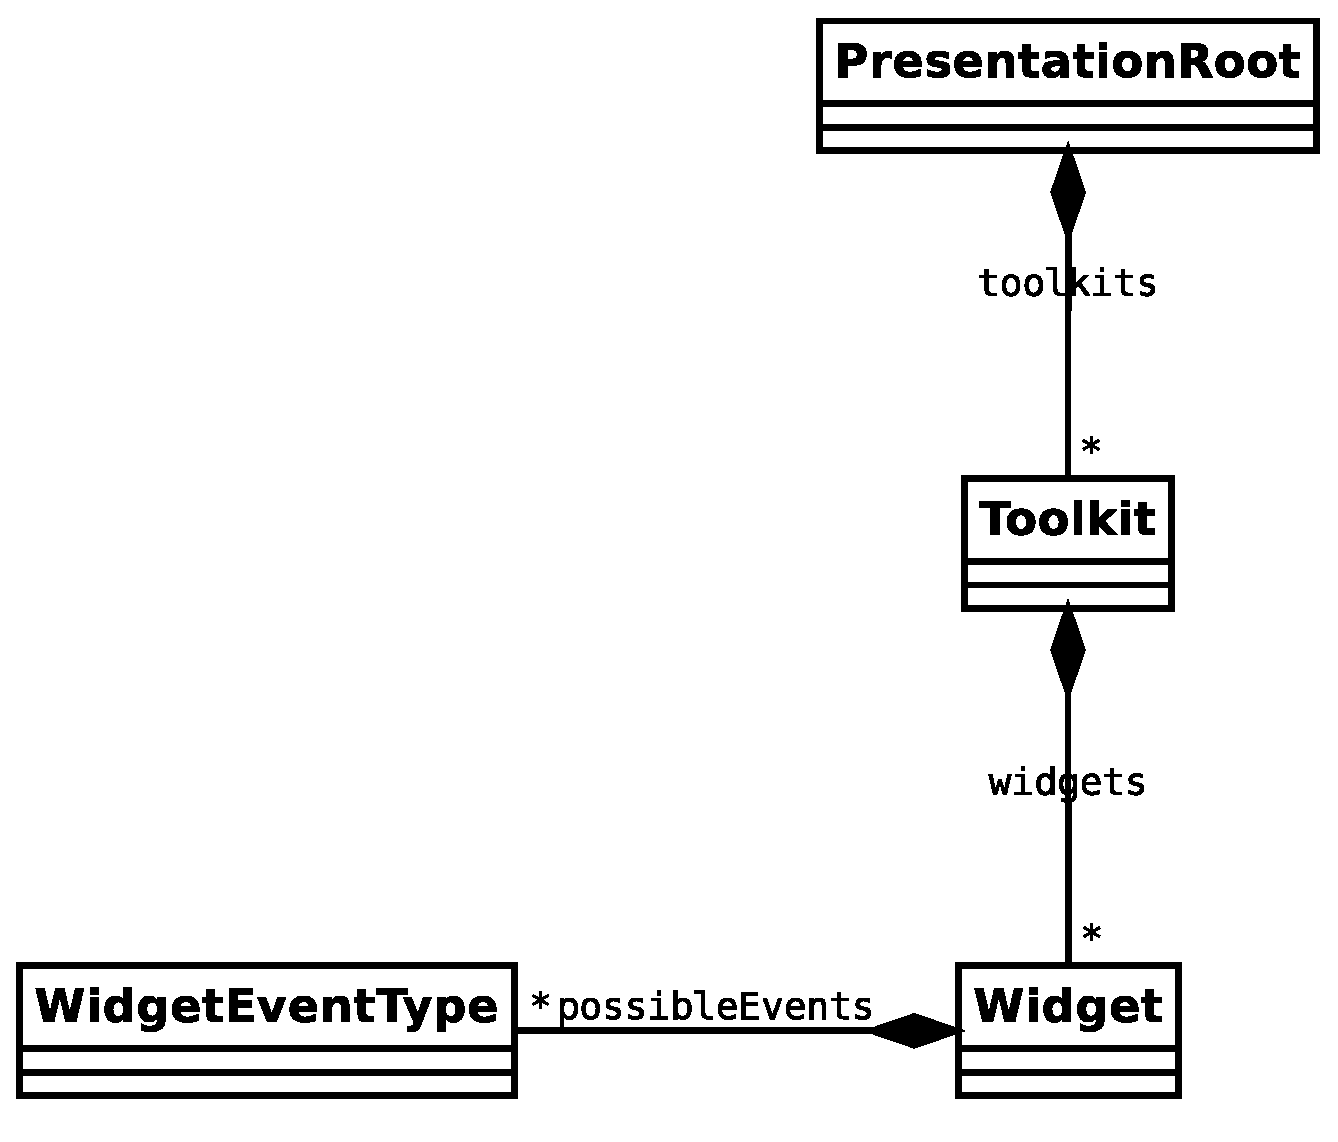
\includegraphics[scale=.3]{img/toolkit.eps}
  \caption{Métamodèle toolkit}
  \label{fig:Métamodèle Toolkit}
\end{figure}
  \item View: représente les concepts liés à la définition des écrans \textsc{ihm}.
\newline
Le package View est construit de la manière suivante:
\newline
\begin{figure}[H]
  \centering
  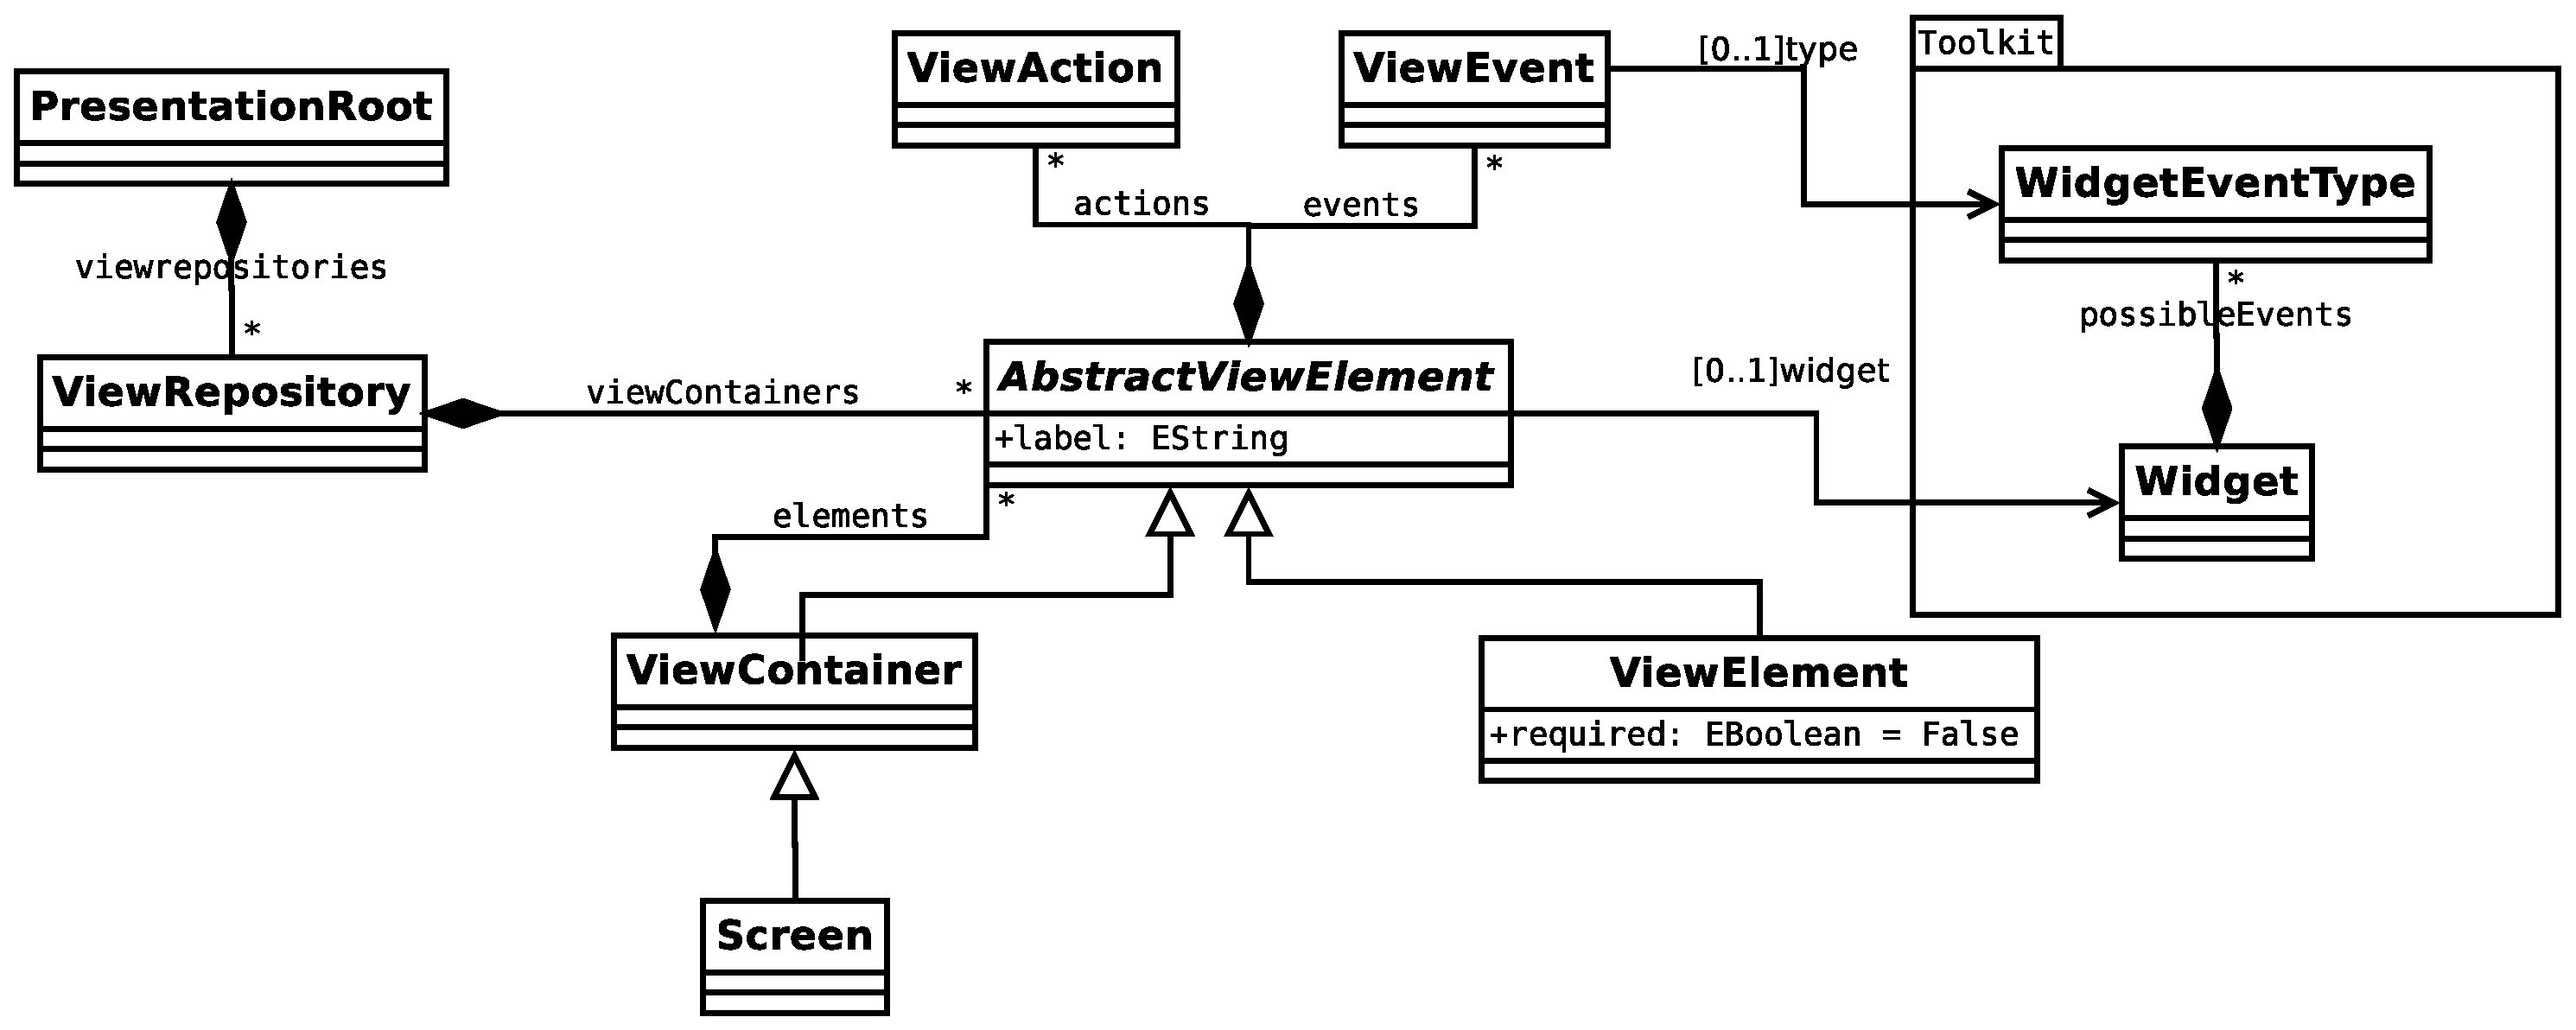
\includegraphics[scale=.3]{img/view.eps}
  \caption{Métamodèle view}
  \label{fig:Métamodèle View}
\end{figure}
  \item Flow: permet d'identifier le comportement dynamique des écrans \textsc{ihm}. Le flow peut être appréhendé comme une sorte de diagramme d'activités.
\newline
Le package Flow est construit de la manière suivante:
\newline
\begin{figure}[H]
  \centering
  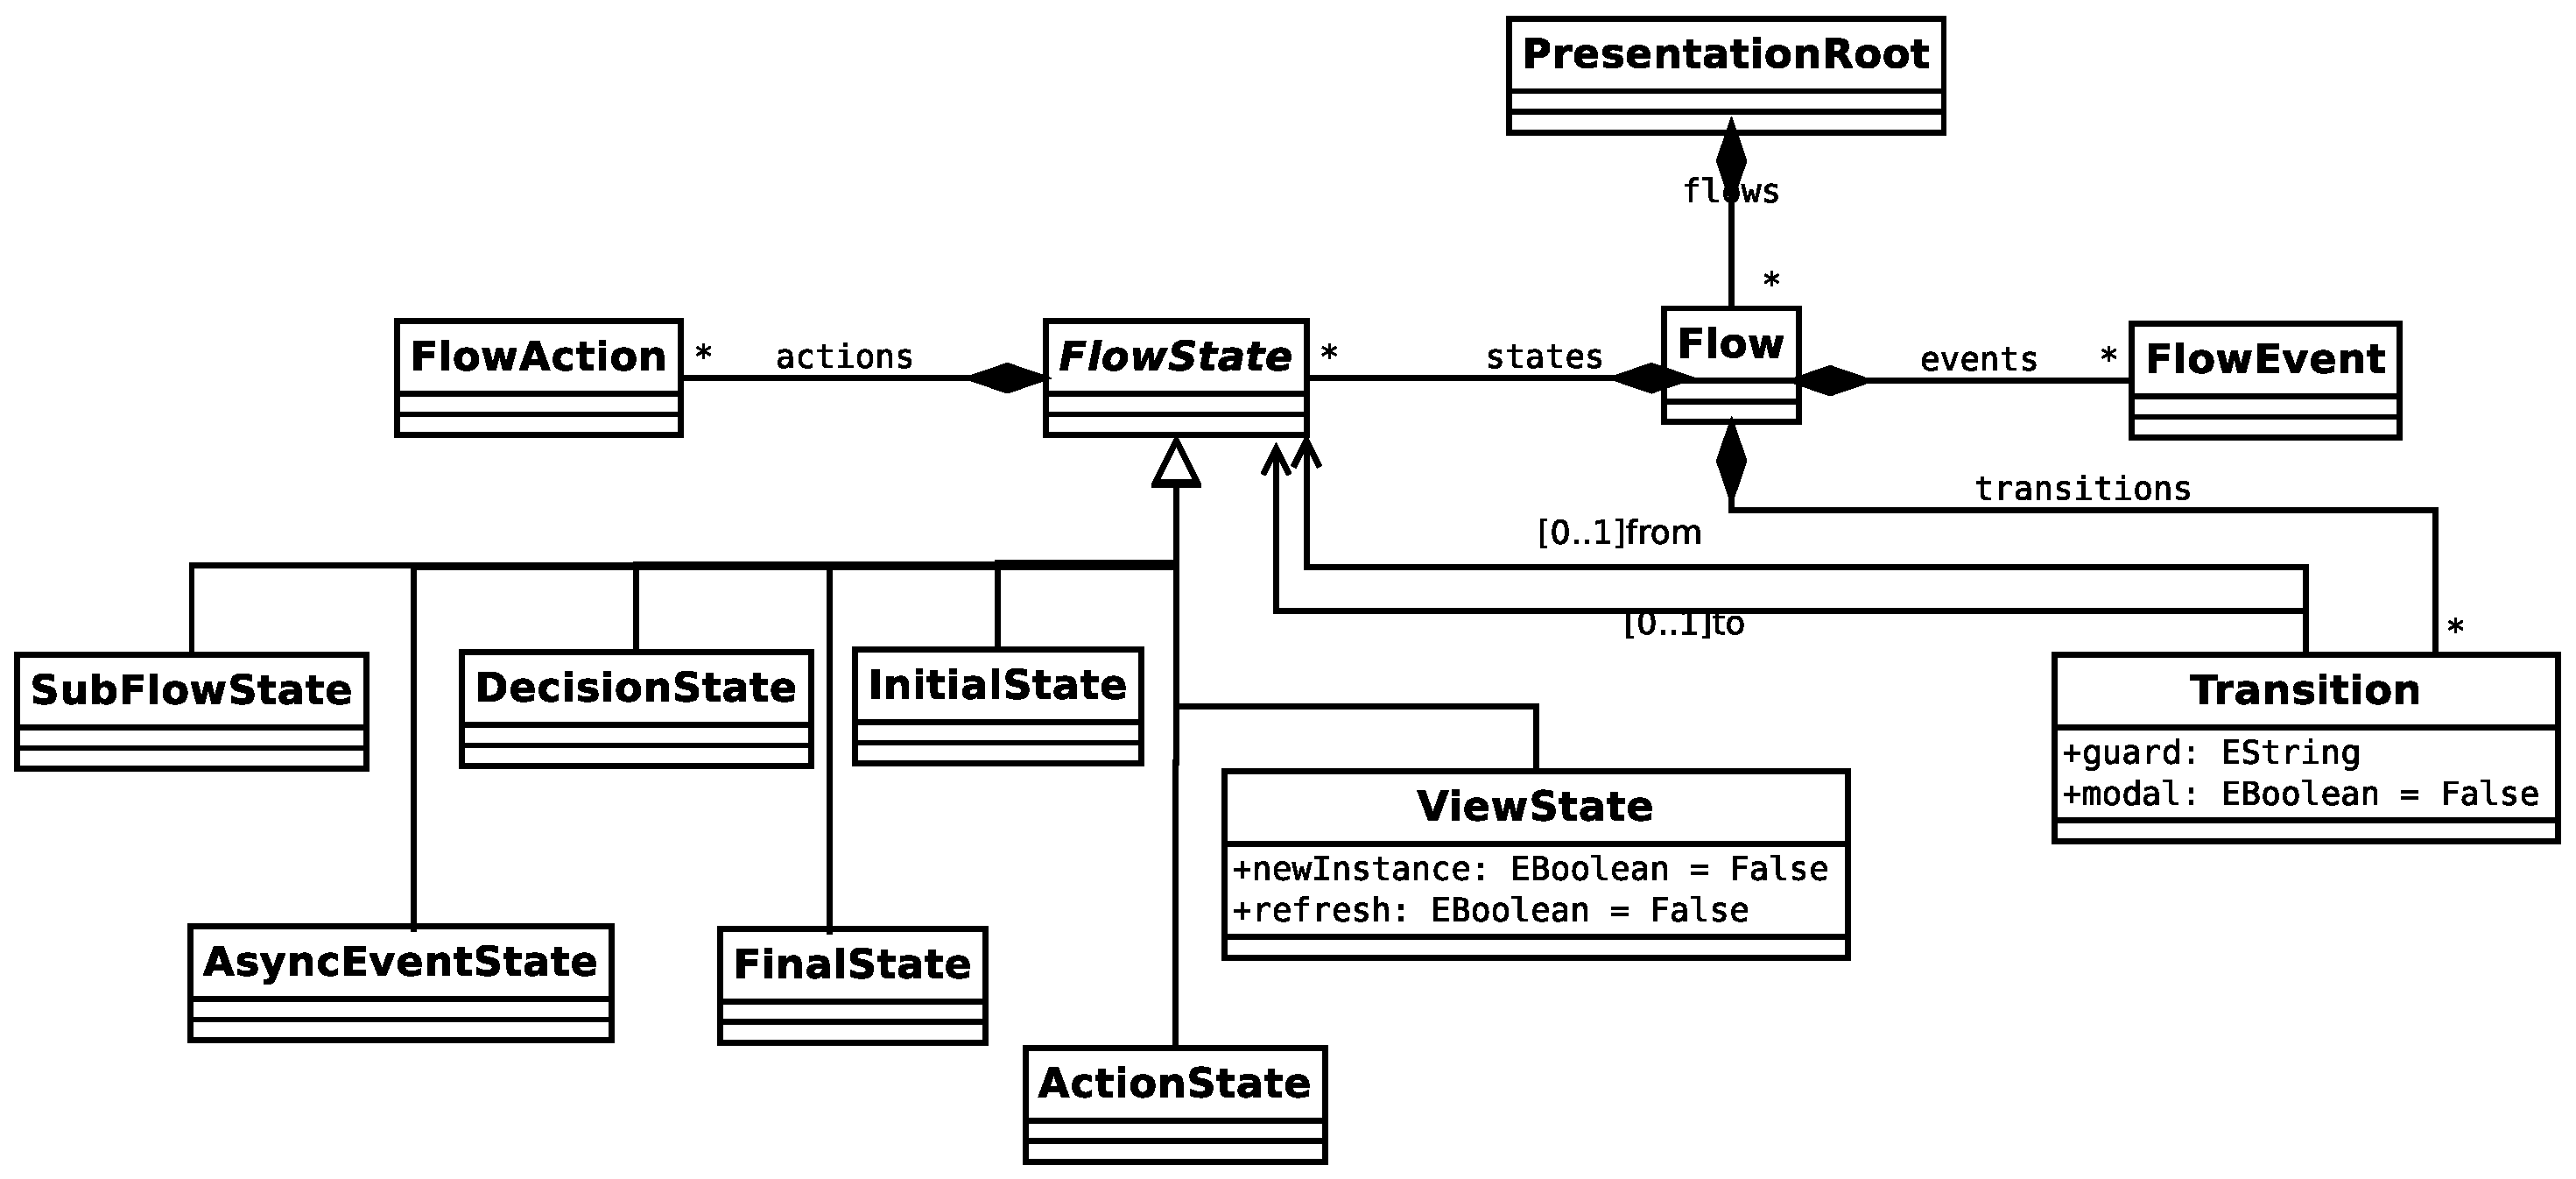
\includegraphics[scale=.3]{img/flow.eps}
  \caption{Métamodèle flow}
  \label{fig:Métamodèle Flow}
\end{figure}
\end{itemize}
\subsection{Le concept cinématique dans \kwplay{}}
blablablablablablablabla
\subsection{Conception du modèle}
La modélisation \textsc{ihm} de l'application prototype \texttt{Play} a été mise en place à l'aide de l'outil acceleo de \texttt{ObeoDesigner}. Le modèle est construit autour des trois principes du métamodèle défini précédemment:
\begin{enumerate}
\item Toolkit: Représente une palette contenant des widgets. Nous avons utilisé le modèle toolkit (par défaut) car il couvre tous les éléments de type "widget web" qui puissent exister (bouton, liste déroulante, champs de saisie, tableau, etc.). Chaque élément "widget" peut lever des événements de type \textit{WidgetEventType}.
\item Flow : Représente la manière dont les écrans de l'application peuvent s'enchaîner. Il décrit le comportement dynamique de l'\textsc{ihm} sous la forme d'enchaînements entre des états.
\item View : Permet de représenter tous les éléments graphiques d'une interface utilisateur. Les views sont liées aux widgets afin de préciser leur type. Par exemple: un viewElement nom est associé au widget "TextField". 

%Cependant, les modèles flow et views ont été conçus de façon conforme aux écrans et à leur enchaînement au niveau de l'application play créée.

\end{enumerate}				


\subsection{Génération du code}

\subsection{Résultats obtenus}
